\documentclass[UTF8]{ctexart}
\usepackage{titlesec}
\usepackage{fancyhdr}
\usepackage{geometry}
\usepackage{listings}
\usepackage{xcolor}
\usepackage{graphicx}

\geometry{left=1.0in,right=1.0in,top=0.3in,bottom=0.3in}

\pagestyle{fancy}
\fancyhf{} 
\ctexset{
    section={
        format=\raggedright
    }
}

\ctexset{
    section={
        format=\raggedright\Large\bfseries
    },
    subsection={
        format=\raggedright\normalsize
    }
}

\lstset{
    language=C++, 
    basicstyle=\ttfamily\small, % 字体样式和大小
    keywordstyle=\color{blue}, % 关键字颜色
    commentstyle=\color{gray}, % 注释颜色
    stringstyle=\color{red}, % 字符串颜色
    numbers=left, % 显示行号
    numberstyle=\tiny\color{gray}, % 行号样式
    frame=single, % 代码框
    breaklines=true, % 自动换行
    captionpos=b % 标题位置
}



\begin{document}

\title{\vspace{0cm}带权中位数实验报告}
\author{程远2234412848}
\date{}
\maketitle
\tableofcontents
\newpage

\section{问题描述}
在统计学中,中位数是排序后居于数据集中心的值,而在带权数据集中,每个元素还具有一个权重。在本实验中,目标是设计并实现一个算法,能够在时间复杂度为O(n)
的情况下找到一组数据的带权中位数。所谓带权中位数,是指一个值,使得其左侧的所有元素的总权重不超过0.5,且其右侧的所有元素的总权重也不超过0.5。

\section{问题分析}
为了在线性时间内找到带权中位数,我们需要避免传统的排序操作(时间复杂度为O(nlogn))。为此,可以采用“中位数的中位数”算法(Median of Medians,线性时间选择中也有用到)
,可在最坏情况下保证 O(n) 的时间复杂度。中位数的中位数算法的基本思想是,通过不断地将数组分组并在组内寻找中位数,最终得到一个接近真正中位数的枢轴,
从而将数据集分为两部分。


\section{算法设计与复杂度分析}
\subsection{分组与排序}
对于一个包含n个元素的数组。算法首先将数组划分为几个小组,每组包含5个元素,则有$⌈n/5⌉$个小组。
每组内需要对这5个元素进行排序,对5个元素进行排序的复杂度为 $O(1)$,$⌈n/5⌉$个小组的总体排序耗时为:$O(⌈n/5⌉)×O(1)=O(n)$。

\subsection{递归找中位数的中位数}
找到每个小组的中位数后,再寻找每个小组中位数构成的数组的中位数,称为“中位数的中位数”,用作下一步分割的枢轴。
现在有$⌈n/5⌉$个中位数,将这些中位数再递归调用该算法,以找到些中位数的中位数。
设递归求解时间为$T(n)$,因为每组有5个元素,因此递归规模为$⌈n/5⌉$个元素。递归求解的时间为$T(n/5)$。

\subsection{分割}
使用“中位数的中位数”作为枢轴,将数组划分为左右两部分。分割过程中遍历每个元素并与枢轴比较,时间复杂度为$O(n)$。

\subsection{递归继续选择}
分割后,只需要在其中一侧递归查找带权中位数。课本线性时间选择算法部分已经证明,
枢轴至少会将数组划分为一个占比约为30\%和一个占比约为70\%的两部分.每次递归时,
只需要处理较小的部分,即最多70\%的数据。因此,递归的规模减小为 
$0.7n$,在最坏情况下,递归过程会逐步缩小为以下递归关系:
$T(n)=T(n/5)+T(0.7n)+O(n)$

\subsection{时间复杂度的递归公式解}
为了简化该公式,可以采用渐进分析法求解:代入 $T(n)=T(n/5)+T(0.7n)+O(n)$,可以递归展开多次。
假设在每层的复杂度为 $O(n)$,可以估计出递归深度的上限为 $O(logn)$。
但由于每次缩小的规模为 $(1−0.3)n$,随着递归层数的增加,划分部分快速收敛于零,因此
$T(n)$ 级数为一个几何级数,整体复杂度最终收敛为$O(n)$。


\section{算法实现}
\subsection{数据结构与自定义比较函数}
\begin{lstlisting}
struct UniElement //储存数字+权值
{
    int number;
    double weight;
    UniElement(int n = -1, double w = 0) : number(n), weight(w) {}
};

bool compareByNumber(const UniElement& a, const UniElement& b) 
{
    return a.number < b.number;
}

    
\end{lstlisting}

\subsection{求中位数的中位数}
\begin{lstlisting}
//求中位数的中位数的函数,用来计算划分位置
int medianOfMedians(int start, int end, vector<UniElement>& elements) 
{
    if (end - start < 5) //递归结束
    {
        sort(elements.begin() + start, elements.begin() + end + 1, compareByNumber);
        return elements[(start + end) / 2].number;
    }
    int numMedians = 0;
    for (int i = start; i <= end; i += 5) //找到每五个数的中位数,并放到向量头部,方便递归处理
    {
        int groupEnd = min(i + 5, end + 1);
        sort(elements.begin() + i, elements.begin() + groupEnd, compareByNumber);
        swap(elements[start + numMedians], elements[(groupEnd + i) / 2]);
        numMedians++;
    }
    return medianOfMedians(start, start + numMedians - 1, elements);
}

\subsection{划分函数}
\begin{lstlisting}
//将数据分成枢轴左右两部分
int partition(int start, int end, vector<UniElement>& elements) 
{
    if (start == end) 
    {
        return start;
    }
    int median = medianOfMedians(start, end, elements);
    int medianIndex = 0;
    for (int i = start; i <= end; i++) 
    {
        if (elements[i].number == median) 
        {
            medianIndex = i;
            break;
        }
    }
    swap(elements[medianIndex], elements[end]); //将枢轴移到向量末尾,方便用循环进行划分
    int storeIndex = start; //记录当前分界线
    for (int i = start; i < end; i++) {
        if (elements[i].number < median) {
            swap(elements[i], elements[storeIndex]);
            storeIndex++;
        }
    }
    swap(elements[storeIndex], elements[end]); //枢轴回位
    return storeIndex; //此时的分界线即为枢轴位置
}
\end{lstlisting}

\subsection{寻找带权平均数的函数}
\begin{lstlisting}
// 计算带权中位数
void WeightMedian(int length, vector<int>& numbers, vector<double>& weights, int index = 0) 
{
    index++; //index已经被我优化掉了,此处是为了防止moodle卡unused variable编译不通过
    vector<UniElement> elements;
    for (int i = 0; i < length; i++) 
    {
        elements.emplace_back(numbers[i], weights[i]);
    }
    int start = 0, end = length - 1; //start,end比length,index好用不少
    double leftWeight = 0.0;
    while (start <= end) //我采用了循环,也可以递归,区别不大
    {
        int pivotIndex = partition(start, end, elements);
        leftWeight = 0.0;
        for (int i = 0; i < pivotIndex; i++)
        {
            leftWeight += elements[i].weight;
        }
        double pivotWeight = elements[pivotIndex].weight;
        double rightWeight = 1.0 - leftWeight - pivotWeight;
        if (leftWeight <= 0.5 && rightWeight <= 0.5) //符合带权中位数要求
        {
            cout << elements[pivotIndex].number << endl;
            return;
        } 
        else if (leftWeight > 0.5) //说明带权中位数在左侧
        {
            end = pivotIndex - 1;
        } 
        else //说明带权中位数在右侧
        { 
            start = pivotIndex + 1;
        }
    }
}
\end{lstlisting}

\section{运行结果}
通过moodle上所有用例
\begin{figure}[htbp]
    \centering
    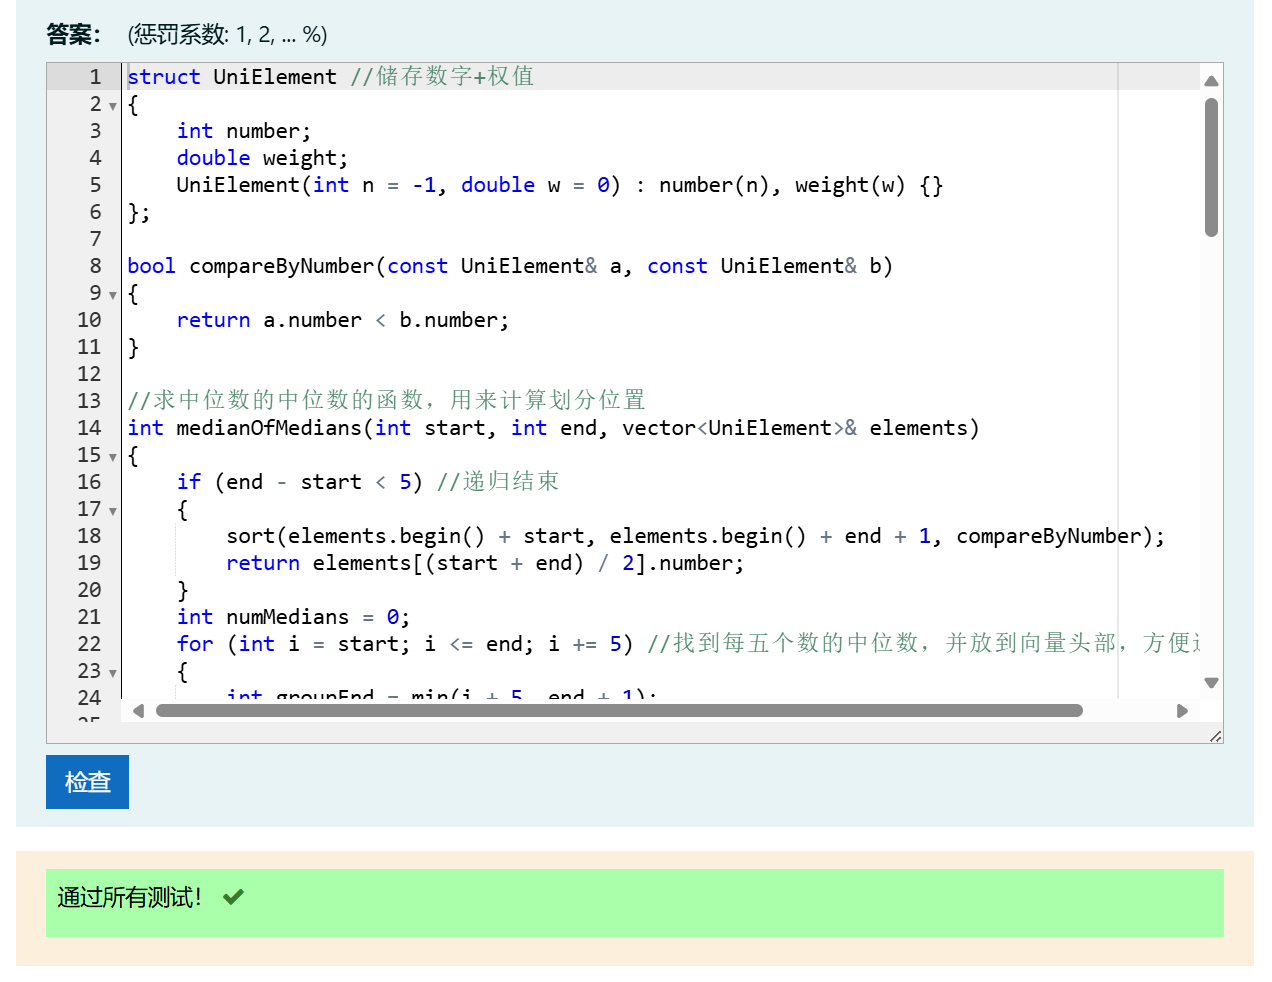
\includegraphics[width=1\textwidth]{moodle1.png}
\end{figure}

\newpage
通过了同学的一些奇怪用例
\begin{figure}[htbp]
    \centering
    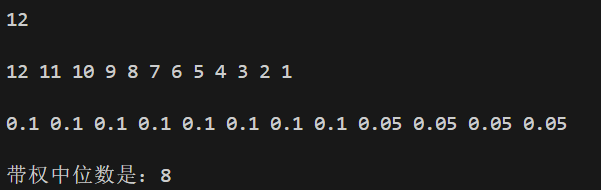
\includegraphics[width=1\textwidth]{12.png}
\end{figure}
\begin{figure}[htbp]
    \centering
    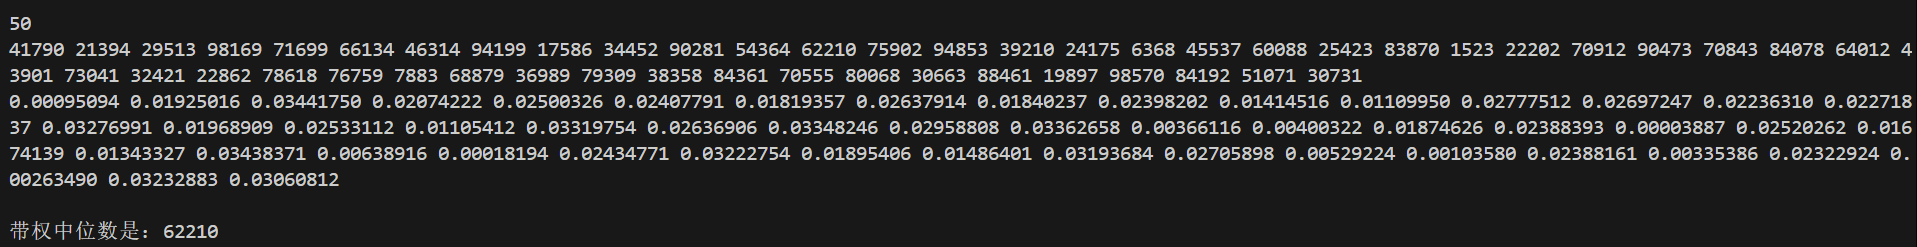
\includegraphics[width=1\textwidth]{50.png}
\end{figure}

\section{反思与改进}
在数据规模过大时,递归可能会导致栈溢出,后续优化可以考虑用迭代代替递归。
可以研究支持其他统计量的计算(如带权平均数或带权分位数)的通用框架。未来可以考虑加入选项,
计算其他带权统计量,以拓展算法的适用范围。
\end{document}